\chapter{设备选型及稳定性校验}

\section{母线的选取}
母线选择应按正常工作的负荷电流考虑,这种正常工作的电流根据不同的工作条件又分为按最大长期工作电流(延续半小时以上)和按经济电流密度两种情况。本设计采用按最大长期工作电流选择母线截面。此外,再按短路条件进行校验。对于$35kV$电压以上的母线,还应按限制电晕电压的要求考虑母线截面的大小。
\subsection{按最大长期工作电流选择母线截面}
根据正常工作下持续发热容许温升$\boldsymbol{\tau }_{\boldsymbol{al}}$的限制,按条件应使最大长期工作电流小于$\boldsymbol{I}_{\boldsymbol{al}}$即:
$$
\boldsymbol{I}_{\boldsymbol{al}}\ge \boldsymbol{I}_{\boldsymbol{w}.\boldsymbol{max}}\label{key}
$$
式中:$\boldsymbol{I}_{\boldsymbol{al}}$为相应于母线工作的环境温度和其放置方式(如矩形母线平放或竖放)下,母线长期容许电流值;$I_{w.max}$为母线在电路中的最大长期工作电流。

对于牵引变压器,应考虑在紧密运行、越区供电(相邻变电所发生故障)等条件下,变压器的长期(1$\sim$2小时)允许过载能力,一般应考虑变压器的额定电流($I_{Nwmax}$)。对于通过式牵引变电所的干功率母线,最大电流($I_{w.max}$)的计算应基于系统中可能出现的最大电流分布。

必须指出,当按照发热条件来验证日照导体(室外)的负荷承载能力时,应该考虑日照的影响。导体的最高温度应等于当地最大日照时的最高空气温度,再加上负荷引起的温升以及来自日照的额外温升。通常,日照强度取$10{W/m^2}$,风速取$0.5 m/s$(室内导体不受日照影响)。根据表格,电流$I_{al}$是在环境温度为25℃时制定的。当实际环境温度不等于25℃时,需要使用修正系数$K_\theta$进行校正,$K_\theta$的值可以按以下方式计算:
$$
K_{\theta}=\sqrt{\frac{\theta _{al}-t}{\theta _{al}-25}}
$$
$$
I_t=K_{\theta}I_{al}
$$
式中:$\theta_{al}$为运行的允许温度,对室外有日照时日$\theta_{al}$=80℃,室内取70℃; t为实际环境温度(℃); $I_t$为实际环境温度t时的容许电流。

母线迭代:
\begin{align}
	I_{w\max}&=1.3I_N\notag
	\\
	&=1.3\times \frac{S}{\sqrt{3}U_N}\notag
	\\
	&=1.3\times \frac{31.5}{\sqrt{3}\times 35}\notag
	\\
	&=675\left( A \right) 
\end{align}

\subsection{按短路条件校验母线的热稳定性}
根据上述正常工作条件确定的母线截面,假定为$S$,则在短路热稳定性的校验时,应按:
$$
A_h=A_s+\frac{1}{S^2}(Q_p+Q_{np})
$$
$$
\theta _s=\theta _0=(\frac{I_w}{I_{al}})(Q_p+Q_{mp})A_z
$$

求出发热系数$A_h$,并从相应材料的$A_\theta=f(\theta)$得到$\theta_h$,必须使$\theta_h≤\theta_{max}$其中($\theta_{max}$为导体短时最大允许发热温度)。

如按最大长期工作电流选择的母线截面不能满足短路发热稳定性要求,则在满足热稳定的前提下,很容易得到母线的最小容许截面$S_{min}$,即:
\begin{align}
	S\sqrt{\frac{Q_k}{A_h-A_s}}\frac{1}{C}\sqrt{Q_k}\frac{1}{C}\sqrt{Q_p+Q_{np}}_{min}\label{math}
\end{align}
\ref{math}式中:C为与母线材料及其发热温度有关的系数,其值如表\ref{tab:线材料及其发热温度有关的系数}所示:
\begin{table}[h]
	\centering
	\renewcommand\arraystretch{2}
	\caption{线材料及其发热温度有关的系数}
	\label{tab:线材料及其发热温度有关的系数}
	\begin{tabular}{ccccccccccc}
		\hline
		起始温度 & 40  & 45  & 50  & 55  & 60  & 65  & 70  & 75  & 80  & 90  \\ \hline
		铝材导体 & 99  & 97  & 95  & 93  & 91  & 89  & 87  & 85  & 83  & 79  \\ \hline
		钢材导体 & 186 & 183 & 181 & 179 & 176 & 174 & 171 & 169 & 165 & 161 \\ \hline
	\end{tabular}
\end{table}
要求短路最终温度$\theta_z$,应先求出起始温度$\theta_s$。再依照$\theta_z$,利用曲线$A_\theta =f(\theta)$,找出对应的$A_s$值。再利用公式$\frac{1}{S^2}Q_d=A_z-A_s$求出$A_z$,最后再利用曲线$A_\theta =f(\theta)$,找出对应的最终温度$\theta_z$。
\begin{align}
\theta _s=\theta _0+\left( \frac{I_{max}}{I_{x_{xu}}} \right) ^2\times (\theta _{x_{xu}}-\theta _0)=\left( \frac{32.02}{156} \right) ^2\times \left( 70-25 \right) =1.90\label{key}
\end{align}
常见材料的$\theta_s$曲线如\ref{材料及其发热温度曲线}所示:
\begin{figure}[h]
	\centering
	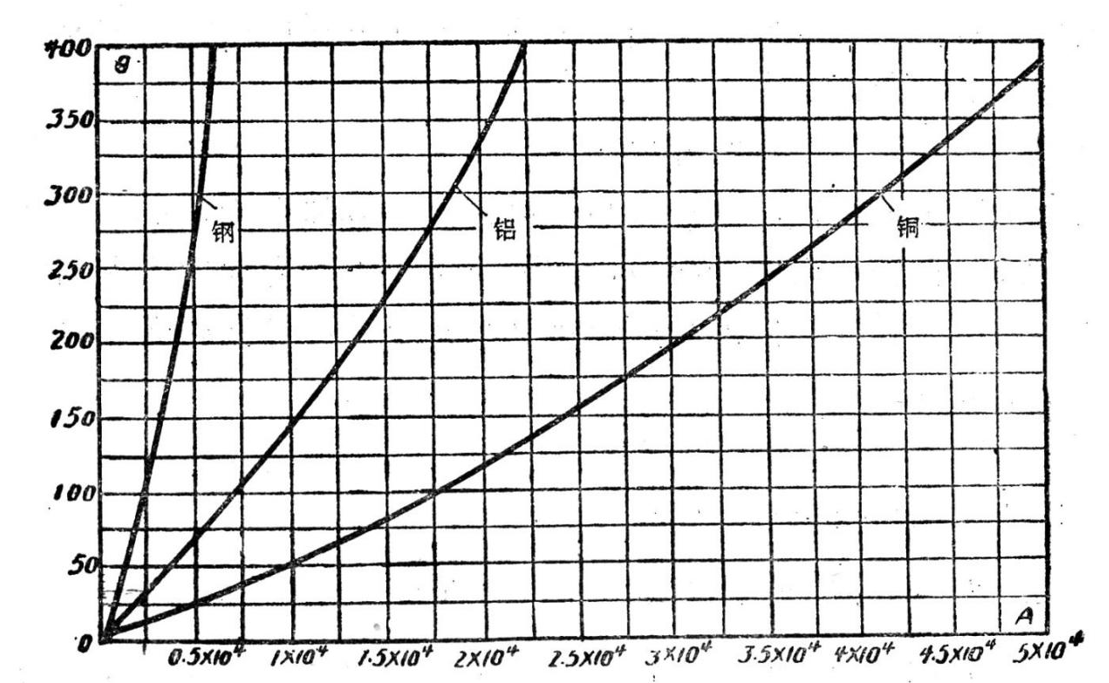
\includegraphics[width=0.8\textwidth]{材料及其发热温度曲线.png}
	\caption{常见材料的$\theta_s$曲线}
	\label{材料及其发热温度曲线}
\end{figure}

检验母线短路热稳定性:
\begin{align}
	\theta _n&=\theta _0+\left( \frac{I_{w.\max}}{I_{a1}} \right) ^2\left( \theta _{a1}-\theta _0 \right) \notag
	\\
	&=25+\left( \frac{675}{703} \right) ^2\times \left( 70-25 \right) \notag
	\\
	&=66.5℃
\end{align}

短路电流计算时间:$t_{ca}=t_{pr}+t_{br}=0.2+0.25=0.45$

短路电流热效应:
\begin{align}
			Q_k&=Q_p+Q_{rp}
			\\
			Q_p&=\frac{3.489^2+10\times 3.489^2+3.489^2}{12}\times 0.4=4.869\left( kA^2\cdot s \right) 
			\\
			Q_{np}&=3.489^2\times 0.05=0.61\left( kA^2\cdot s \right) 
			\\
			Q_k&=5.48\left( kA^2\cdot s \right) 
\end{align}

查表知:当$\theta_n$=66.5℃时,$$A_\theta=0.5\times10^4$$
$$A_h=0.5\times10^4+\frac{5.479\times10^6}{300^2}=0.506\times10^4$$

查表知:当$A_n=0.506\times10^4$时,
$$\theta_n=70℃<<300℃$$满足热稳定性。

\subsection{按短路条件校验母线的机械稳定性}
检验母线的机械稳定性:

冲击电流$I_{sh}=\sqrt{2}\times1.8\time 3.489=8.88kA$

查表知:$$a=50cm,l=100cm,h=50mm,b=6mm$$
$$\frac{a-b}{b+h}=7.036$$
$$k=1$$

三相短路时的相间电动力:$F^{\left( 3 \right)}=1.73\times \left( 8.88 \right) ^2\times 10^6\times \frac{100}{40}\times 10^{-7}=34.1N$

抗弯模量:$W=\frac{1}{6}\times 0.006\times \left( 0.05 \right) ^2=2.5\times 10^{-6}m^2$

计算应力:$\sigma =\frac{M}{W}=\frac{34.1\times 0.1}{2.5\times 10^{-6}}=1.364\times 10^6Pa$

查表可知铝制母线的允许应力为$69\times10^6Pa>5$,故满足机械稳定性。
\section{电缆选型}
热温度系数:
$$
C=\sqrt{\frac{4.2\times 0.81}{1\times 1.84\times 10^{-6}\times 3.93\times 10^{-3}}\ln \frac{1+1.39\times 10^{-3}\times \left( 250-20 \right)}{1+3.93\times 10^{-2}\times \left( 66.5-20 \right)}}\times 10^{-2}=150
$$

最小截面:
$$
S_{\min}=\frac{\sqrt{5.479}}{150}\times 10^3=15.6mm^2<150mm^2
$$

设计采用$150mm^2$交联聚乙烯绝缘电力电缆。
\section{断路器的选型}
目前一般使用的断路器类型有:少油断路器、真空断路器、SF6断路器,要根据使用场合和用途选择断路器类型,少油断路器属于通用产品,如果没有特殊要求,一般选少油断路器;真空断路器分合闸时间短、允许动作次数多,一般频繁操作和对动作时间有特殊要求的场合使用;SF6断路器绝缘性能好,一般用于高压系统中。

$I_{w.max}=675A$应该需要满足$I_N\geqslant I_{w.\max}=675A\ U_N\geqslant U_{w}=35kV$

按照断路电流选择可以选择$Z_N-35$真空断路器。

热稳定性检验:

\begin{align}
		I_{t}^{2}\cdot t&\geqslant Q_k\notag
		\\
		Q_k&=5.479\left( kA\cdot s \right) \notag
		\\
		I_t&=16A\notag
		\\
		t&=4s\notag
\end{align}

带入计算可知满足要求。

动稳定性检验:$i_{Nck}=17kA>i_{sh}=8.88kA$,满足要求。
\section{电压互感器的选型}
所选电压互感器的额定一次侧电压必须与互感器接入点所在电网的额定电压相匹配。这一选择应基于测量监视点的电压等级来确定。要求互感器的原边电压满足以下条件:
$$1.1U_e>U_1>0.9U_e$$

所选电压互感器的额定二次侧电压应与测量仪表和继电器的额定电压相匹配,通常为$100V$或$100/\sqrt{3}V$。在本例中,选择了型号为JDJ-35的电压互感器,其准确度等级为0.5,额定容量为$150kVA$。

对于电压等级小于等于$35kV$的情况,通常采用油浸式普通结构或环氧树脂浇注干式结构;而对于电压等级大于等于$100kV$的情况,采用串级式电压互感器。因此,此处选择了油浸式普通结构或环氧树脂浇注干式结构的电压互感器。

在选择精确度等级时,通常可以依据以下原则确定精确度等级:用于计量(如接电能表)的精确度等级为0.5;用于供给监视用电能表、功率表或发电厂电压继电器的等级为1;而用于供给监视用电压表、电压继电器的等级为3。此外,副边负荷的总和应小于相应精确度等级对应的额定容量。如\ref{tab:电压互感器参数}所示。

\begin{table}[h]
	\centering
	\renewcommand\arraystretch{2}
	\caption{电压互感器参数}
	\label{tab:电压互感器参数}
	\begin{tabular}{|c|ccc|ccc|c|c|}
		\hline
		\multirow{2}{*}{型号} & \multicolumn{3}{c|}{额定电压/kV}                               & \multicolumn{3}{c|}{额定容量/VA}                               & \multirow{2}{*}{最大容量/VA} & \multirow{2}{*}{绝缘形式} \\ \cline{2-7}
		& \multicolumn{1}{c|}{原线圈} & \multicolumn{1}{c|}{副线圈} & 辅助线圈 & \multicolumn{1}{c|}{0.5级} & \multicolumn{1}{c|}{1级}  & 3级  &                          &                       \\ \hline
		JDJ-35              & \multicolumn{1}{c|}{35}  & \multicolumn{1}{c|}{0.1} &      & \multicolumn{1}{c|}{150}  & \multicolumn{1}{c|}{250} & 600 & 1200                     & 油侵式                   \\ \hline
	\end{tabular}
\end{table}


\begin{table}[h]
	\caption{电压互感器二次负荷统计表}
	\centering
	\renewcommand\arraystretch{2}
	\label{tab:电压互感器二次负荷统计表}
	\begin{tabular}{|ccccc|}
		\hline
		\multicolumn{1}{|c|}{\multirow{2}{*}{仪表名称}} & \multicolumn{1}{c|}{\multirow{2}{*}{仪表电压线圈数}} & \multicolumn{1}{c|}{\multirow{2}{*}{仪表总数}} & \multicolumn{2}{c|}{仪表所需功率}          \\ \cline{4-5} 
		\multicolumn{1}{|c|}{}                      & \multicolumn{1}{c|}{}                         & \multicolumn{1}{c|}{}                      & \multicolumn{1}{c|}{功率 VA/个} & 总计/VA \\ \hline
		\multicolumn{1}{|c|}{有功瓦时计}                 & \multicolumn{1}{c|}{2}                        & \multicolumn{1}{c|}{6}                     & \multicolumn{1}{c|}{1.5}     & 9     \\ \hline
		\multicolumn{1}{|c|}{无功电度表}                 & \multicolumn{1}{c|}{2}                        & \multicolumn{1}{c|}{6}                     & \multicolumn{1}{c|}{1.5}     & 9     \\ \hline
		\multicolumn{1}{|c|}{电压表}                   & \multicolumn{1}{c|}{1}                        & \multicolumn{1}{c|}{1}                     & \multicolumn{1}{c|}{4.5}     & 4.5   \\ \hline
		\multicolumn{4}{|c|}{总计}                                                                                                                                                & 22.5  \\ \hline
	\end{tabular}
\end{table}

0.5级电压互感器JDJ − 35额定容量为$150VA$,远大于$22.5VA$,经校验满足容量需求。
\section{电流互感器的选型}
电流互感器的额定一次电压必须与互感器安装处的额定电压一致,它与额定电流应满足:
$$
U_{1N}\ge U_{Nw},I_{1N}\ge I_g
$$

在环境温度条件下,应该尽量使连续通过电流互感器的原边电流接近互感器的额定电流$I_{1N}$。如果电流过大,将会导致误差增加。通常,电流互感器的二次额定电流为5A,这与仪表和继电器的标准电流相匹配。

% Please add the following required packages to your document preamble:
% \usepackage{multirow}
\begin{table}[h]
	\caption{电流互感器参数}
	\renewcommand\arraystretch{2}
	\centering
	\label{tab:电流互感器参数}
	\begin{tabular}{|c|c|c|c|cccc|cc|c|c|}
		\hline
		\multirow{2}{*}{型号} & \multirow{2}{*}{\begin{tabular}[c]{@{}c@{}}额定\\ 电流\\ 比/A\end{tabular}} & \multirow{2}{*}{\begin{tabular}[c]{@{}c@{}}级次\\ 组合\end{tabular}} & \multirow{2}{*}{\begin{tabular}[c]{@{}c@{}}准确\\ 级次\end{tabular}} & \multicolumn{4}{c|}{\begin{tabular}[c]{@{}c@{}}二次\\ 负荷/$\Omega$\end{tabular}} & \multicolumn{2}{c|}{\begin{tabular}[c]{@{}c@{}}10\%\\ 倍数\end{tabular}} & \multirow{2}{*}{\begin{tabular}[c]{@{}c@{}}1秒\\ 热稳\\ 定倍\\ 数$K_t$\end{tabular}} & \multirow{2}{*}{\begin{tabular}[c]{@{}c@{}}动稳\\ 定倍\\ 数$K_u$\end{tabular}} \\ \cline{5-10}
		&  &  &  & \multicolumn{1}{c|}{\begin{tabular}[c]{@{}c@{}}0.5\\ 级\end{tabular}} & \multicolumn{1}{c|}{\begin{tabular}[c]{@{}c@{}}1\\ 级\end{tabular}} & \multicolumn{1}{c|}{\begin{tabular}[c]{@{}c@{}}3\\ 级\end{tabular}} & \begin{tabular}[c]{@{}c@{}}D\\ 级\end{tabular} & \multicolumn{1}{c|}{\begin{tabular}[c]{@{}c@{}}二次\\ 负荷\\ /Ω\end{tabular}} & \begin{tabular}[c]{@{}c@{}}倍\\ 数\end{tabular} &  &  \\ \hline
		\multirow{2}{*}{LCW-35} & \multirow{2}{*}{15$\sim$1000/5} & \multirow{2}{*}{0.5/3} & 0.5 & \multicolumn{1}{c|}{2} & \multicolumn{1}{c|}{4} & \multicolumn{1}{c|}{} &  & \multicolumn{1}{c|}{2} & 20 & 65 & 100 \\ \cline{4-12} 
		&  &  & 3 & \multicolumn{1}{c|}{} & \multicolumn{1}{c|}{} & \multicolumn{1}{c|}{2} & 4 & \multicolumn{1}{c|}{2} & 28 & 65 & 150 \\ \hline
	\end{tabular}
\end{table}

电流互感器的热稳定性要求为下两式之一:
$$
(I_{1n}K_t)^2t\le Q_k
$$
$$
(I_{1n}K_t)^2t\ge I_{\infty}^{2}t_{eq}
$$
式中,$K_t$为互感器热稳定倍数,即热稳定电流与额定一次电流之比,$t$为热稳定电流通过的时间($t=1s$);$I_{1N}$为电流互感器一次侧额定电流。

选择LCW-35,计算检验如下:
\begin{align}
		U_{1N}&\geqslant U_{NW}=35kV
		\\
		I_{1N}&\geqslant I_{W.\max}=675A
		\\
		i_{sh}&=8.88kA
		\\
		Q_k&=5.479\left( kA^2\cdot s \right) 
\end{align}

动稳定检验:
$$
\sqrt{2}I_{1N}\cdot K_{es}=\sqrt{2}\times 0.675\times 150=143.2kA>i_{sh} \;
$$

满足要求。

热稳定检验:
$$
\left( I_{1N}K_t \right) ^2t=\left( 0.675\times 65 \right) ^2\times 1=2851.875kA^2\cdot s>Q_k
$$

满足要求。
\section{隔离开关的选型}
$$
\begin{cases}
	I_{W\cdot \max}&=675A\\
	U_W&=35kV\\
\end{cases}\Longrightarrow GN2-35T/1000
$$

热稳定校验:
$$
i_{es}=70kA>i_{sh}=8.88kA
$$


满足要求。
\section{设备选型汇总}
本章内容通过查阅相关资料,确定断路器、电流互感器、电压互感器、母线、电缆的选型原则。并通过比对各不同型号的电气设备,选择最适合该种情况的设备。此后,结合最大短路电流值等参数,进行动稳定性校验、热稳定性校验等,以保证该设备的选型合理且可以短期适用于短路等极端情况。最终,各电气设备选型结果如表\ref{tab:设备选型汇总表}所示:
\begin{table}[ht]
	\caption{设备选型汇总表}
	\label{tab:设备选型汇总表}
	\renewcommand\arraystretch{2}
	\centering
	\begin{tabular}{|c|c|c|}
		\hline
		设备名称 & 型号 & 数量 \\ \hline
		\multirow{2}{*}{母线} & \multirow{2}{*}{铝母线(LMY型)$50\times 6$} & \multirow{2}{*}{4} \\
		&  &  \\ \hline
		电缆 & 150$mm^2$交联聚乙烯绝缘聚乙烯护套电力电缆 & 1 \\ \hline
		断路器 & ZN-35 & 8 \\ \hline
		电压互感器 & JDJ-35 & 4 \\ \hline
		电流互感器 & LCW-35 & 12 \\ \hline
		隔离开关 & GN2-35T/1000 & 6 \\ \hline
	\end{tabular}
\end{table}

